\chapter{Virtualization and Containerization}

Virtualization and containerization are widely appreciated techniques for distributing multiple instances of applications on single or multiple physical servers. The most important objective of virtualization and containerization is for each instance to generate consistent result, while deploying each instance efficiently and saving the total resource consumption.

\section{Introduction}

One of the major differences between a server (or a server cluster) and a PC is that a server is usually shared among multiple users or applications at the same time. Though working on the same machine, a user would usually want a private working environment not interrupted by other users. In other words, each and every user would want to ``virtually'' work on an independent machine with his own CPU, RAM, I/O, OS, drivers and hard disk storage, despite that the actual hardware is shared with others. This is done through \textit{Virtualization}, which enables running multiple operating systems on a single physical server in an uninterrupted and logically separated manner. The virtually independent computer of such kind is often called a \textit{virtual machine} (VM).

Deploying a new VM would generally consume considerably large amount of time and computational load, because it needs to load the OS in its first startup. Consider a case where there are hundreds of small applications (microservices, as people call them nowadays), each requiring running in a similar but separate environment. Launching a VM for each application can be a solution, but it can be expensive due to the time and resource consumption burden. It would be batter to rather deploy only one VM (or physical server), and put each application in a ``container'' with its own customized drivers and configurations. A container is similar with a VM in the sense that it runs separately from other containers. However, a container is much ``lighter'' than a VM, thus is cheaper to launch and manage. This becomes possible thanks to \textit{containerization}. Since a container contains all the configuration and minimum requirement information of the application, running a container on different platforms would generate consistent result. This has made sharing and fast-deploying of containers very easy and convenient. The similarities and differences of personal PC, VM, and container applications are summarized in Fig. \ref{ch:vac:fig:pcvmcontainersructure}.

As an analogy, think of running an APP as asking a restaurant to prepare a dish. The hardware is corresponding with the kitchen of the restaurant. The OS is corresponding with the cook, who uses the materials in the kitchen to make the dish. The OS needs associated drivers and libraries to run the APP correctly. The drivers and libraries are like the skill set expected from the cook in order to prepare the dish correctly. Therefore, installing and configuring drivers and libraries in the OS is like teaching the cook how the dish should be prepared. Finally, the APP is corresponding with the expected dish.

\begin{figure}
	\centering
	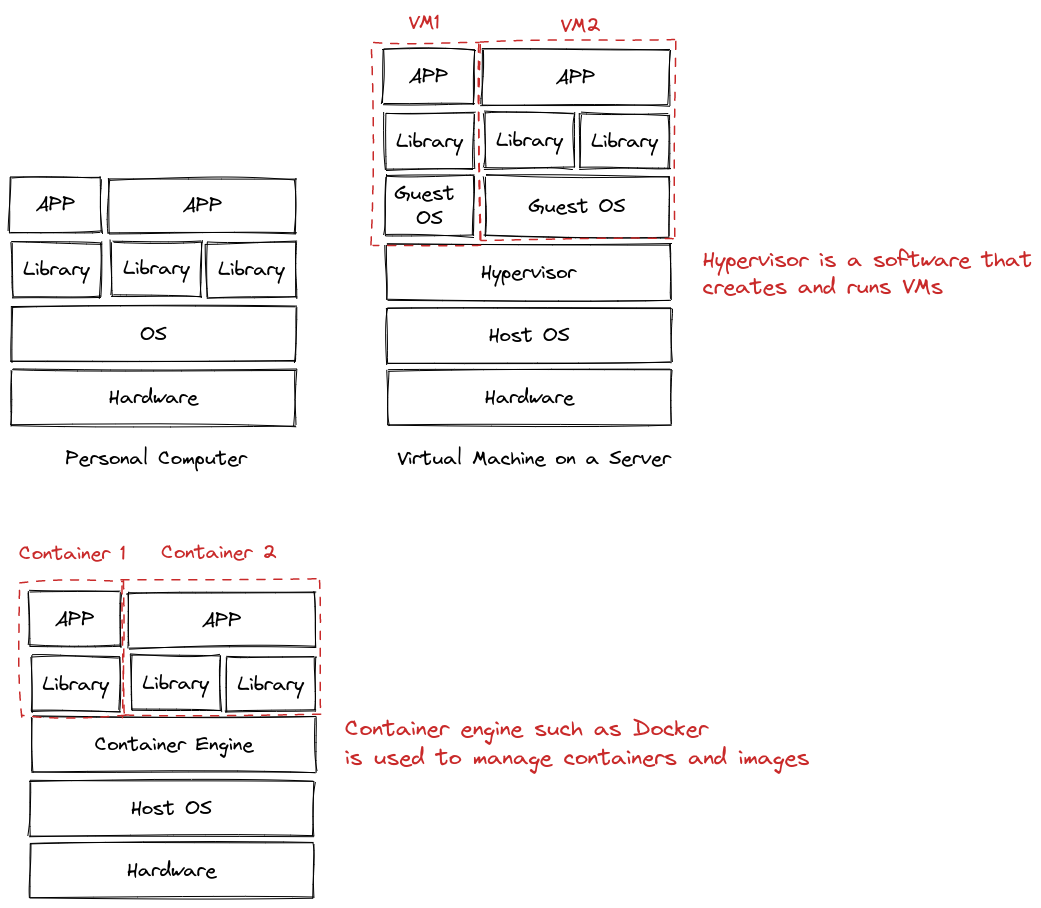
\includegraphics[width=350pt]{chapters/ch-virtualization-and-containerization/figures/pcvmcontainerstructure.png}
	\caption{System architectures of PC, VM and container.} \label{ch:vac:fig:pcvmcontainersructure}
\end{figure}

In the most simple configuration, a dedicated machine is used to run an APP. This is like constructing a dedicated kitchen and hiring a dedicated cook for each dish. The cook is trained to master all necessary skills required for that specific dish, as shown in Fig. \ref{ch:vac:fig:acookinakitchen}.
\begin{figure}
	\centering
	
\includegraphics[width=300pt]{chapters/ch-virtualization-and-containerization/figures/acookinakitchen.png}
	\caption{PC implementation: a cook in a kitchen.} \label{ch:vac:fig:acookinakitchen}
\end{figure}

In a VM implementation, a larger and more capable kitchen is setup in advance as shown in Fig. \ref{ch:vac:fig:manycooksinakitchen}. For each dish, a cook is hired. Each cook is trained with the skills necessary for his assigned dish. All cooks share the same kitchen. This implementation is more efficient than Fig. \ref{ch:vac:fig:acookinakitchen}, as there is no need to scale up the kitchen for a new dish. By sharing the resources among the cooks, the resources in the kitchen can be utilized more effectively.
\begin{figure}
	\centering 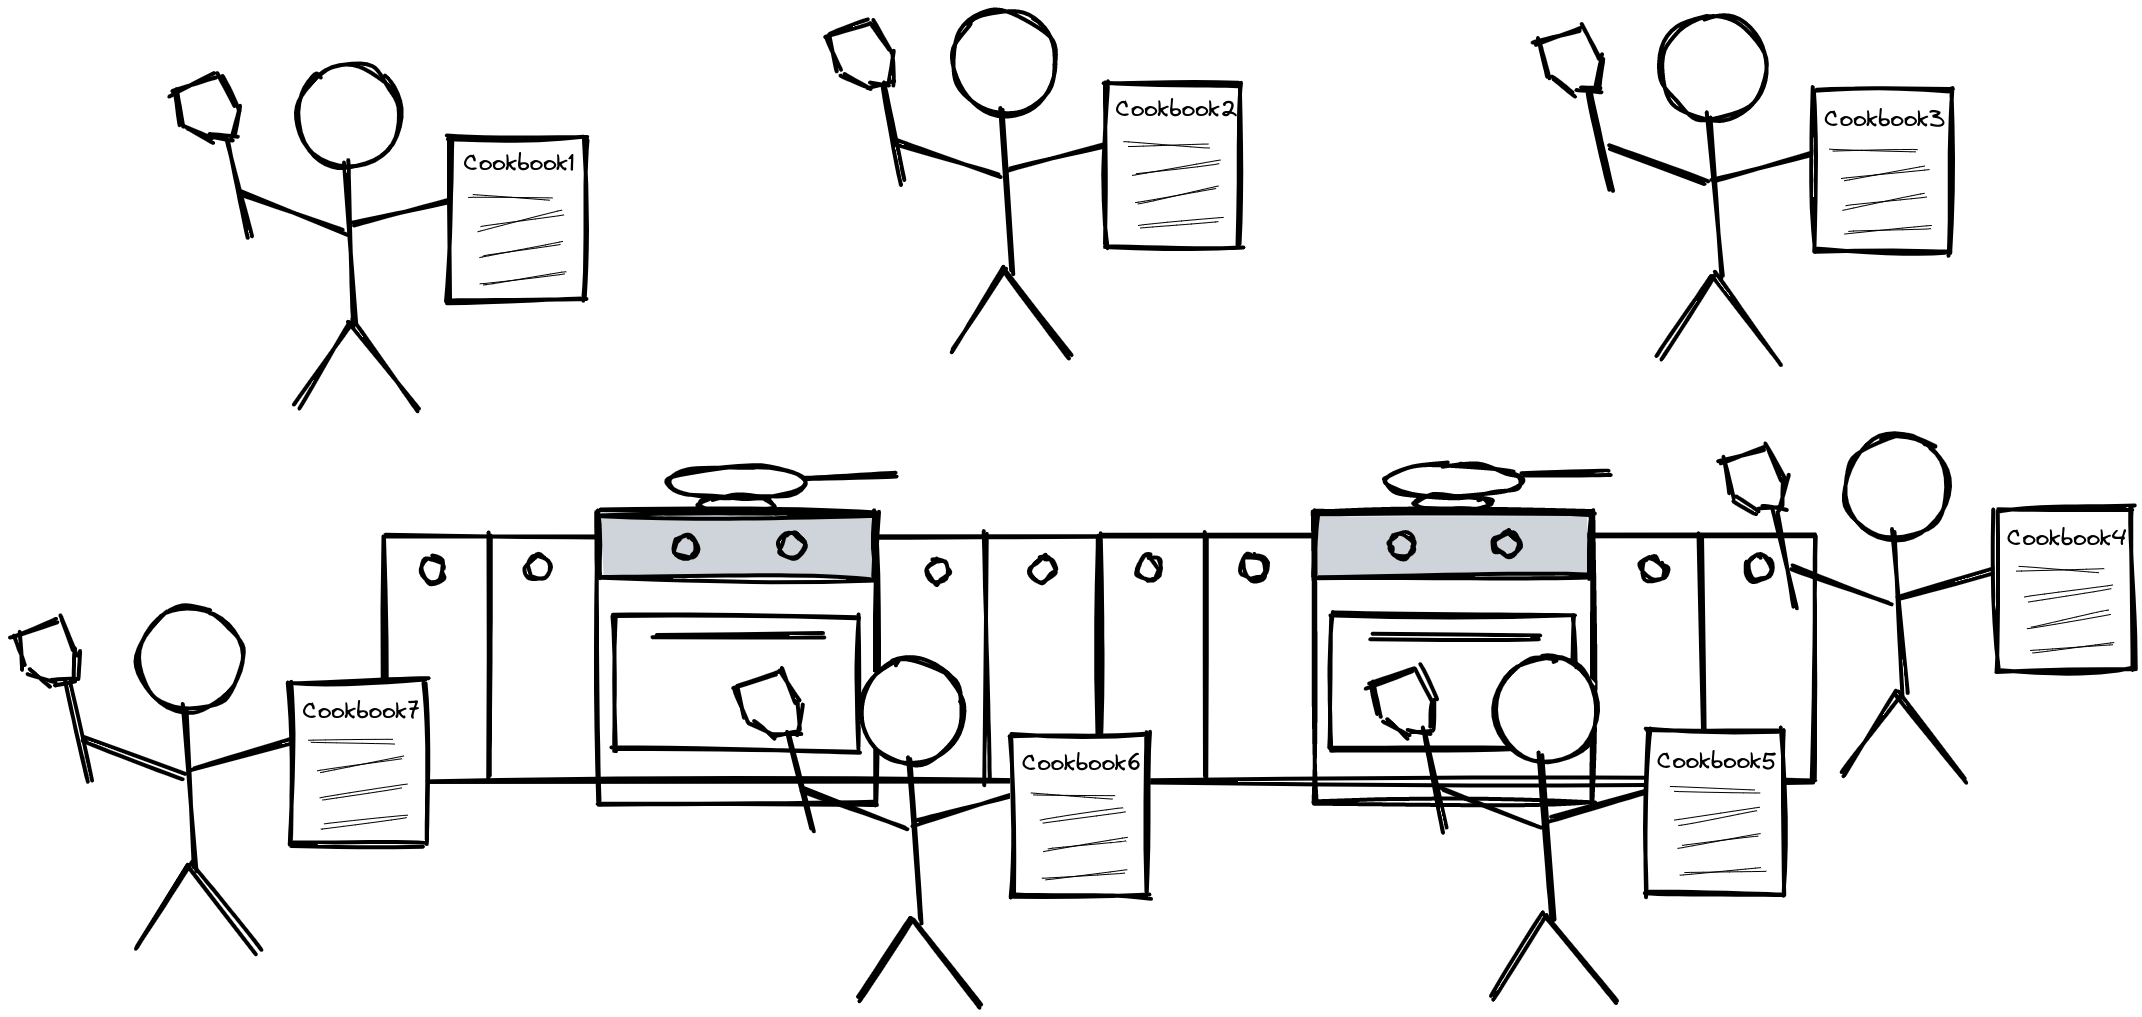
\includegraphics[width=350pt]{chapters/ch-virtualization-and-containerization/figures/manycooksinakitchen.png}
	\caption{VM implementation: many cooks in a kitchen, each with a different cookbook.} \label{ch:vac:fig:manycooksinakitchen}
\end{figure}

While Fig. \ref{ch:vac:fig:manycooksinakitchen} might be a popular practice in many restaurants, it is still too costly to hire a new cook for each different dish. In a containerization implementation, a cook usually handles a category of dishes, as shown in Fig. \ref{ch:vac:fig:multitaskcook}. Of course, each dish will stay in its own fry-pan in an isolated way. For each dish, its receipt is provided that contains everything needed to prepare the dish consistently. As long as the cook is good at multi-tasking, Fig. \ref{ch:vac:fig:multitaskcook} is a more efficient implementation than Fig. \ref{ch:vac:fig:acookinakitchen}.

\begin{figure}
	\centering
	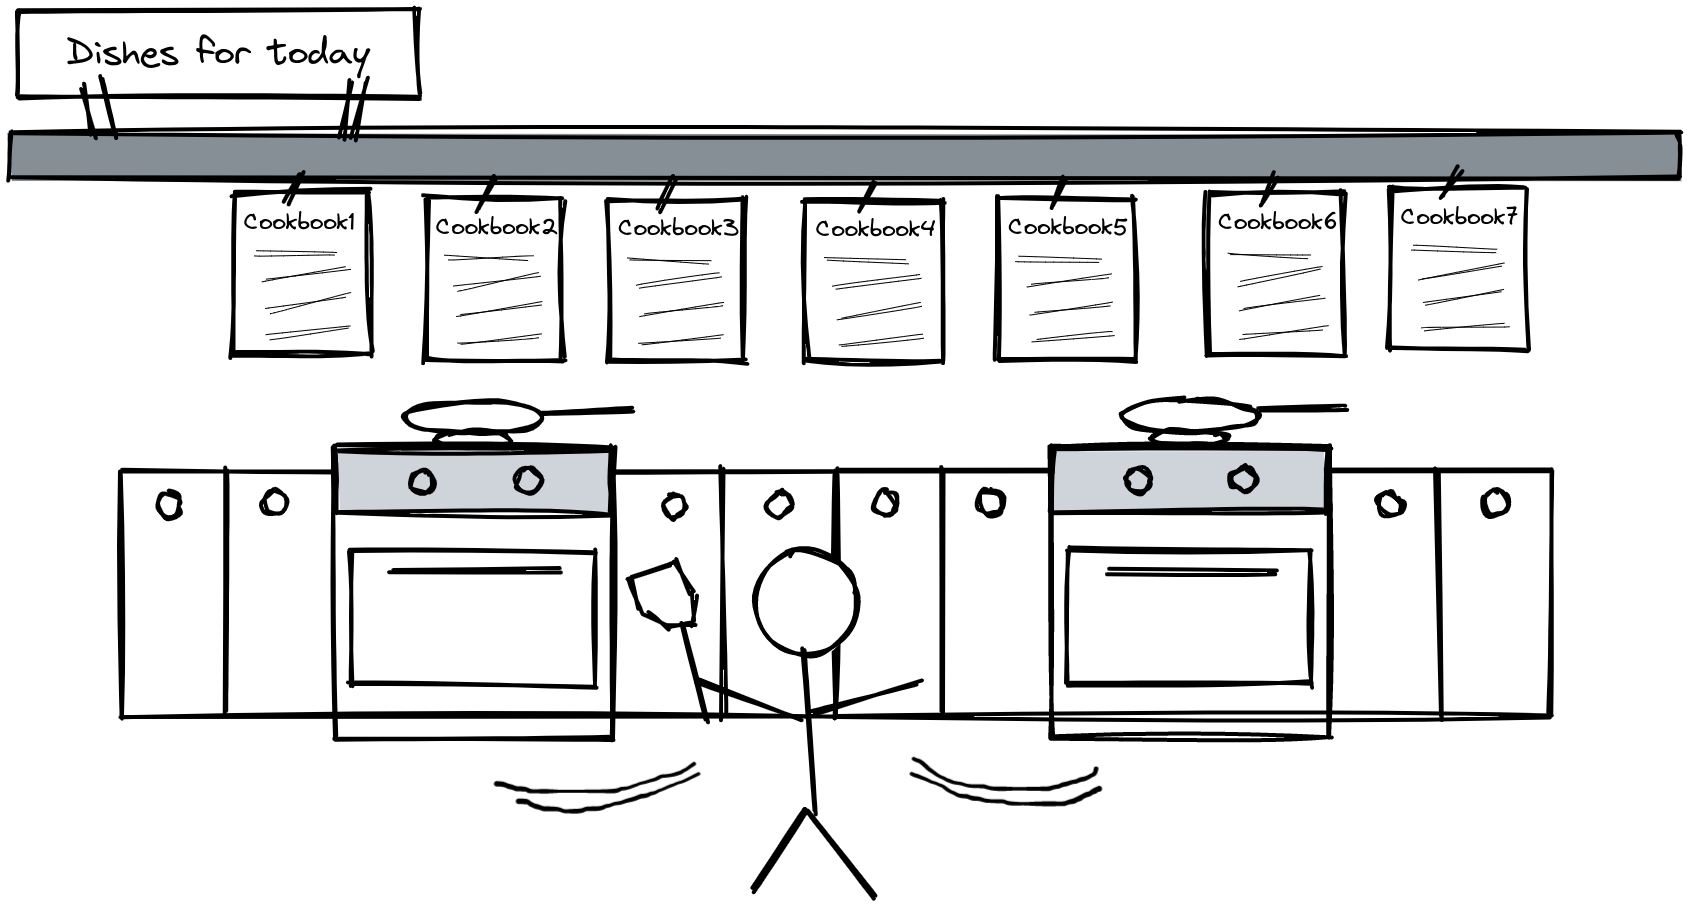
\includegraphics[width=350pt]{chapters/ch-virtualization-and-containerization/figures/multitaskcook.png}
	\caption{Container implementation: one in a kitchen, handling multiple dishes, each has a cookbook and stays in its own pan.} \label{ch:vac:fig:multitaskcook}
\end{figure}

Just like a receipt guaranteeing the consistency of dishes, in containerization, an ``image'' guarantees the consistent performance of container instances. An image is basically a collection of prerequisites and configurations, from where a container can be launched quickly and conveniently. Images can be shared among machines to replicate the containers, even if the machines use different OS.

\section{Virtualization and Containerization}
...

\section{Docker Container} \label{ch:vac:sec:dc}

Before moving forward to the introduction of containerization approaches, it is important to briefly explain the following 3 terms what would be frequently mentioned in the remaining of this chapter: container runtime, container engine, and container orchestration. 

Container runtime refers to the backend software that actually runs the containers. One of the widely used container runtimes is ``containerd''. Other container runtime examples include ``runc''. Container engine is the interface for a user or software to manage images and containers. One of the widely used container engines is ``docker''. Alternatives to docker include ``podman''. Finally, container orchestration is the software that smartly deploy, monitor, restart, and terminate the containers on servers. It is often able to automatically scale up and down the number of running containers based on the loads, balance the API calls made to the containers. One of the most widely used container orchestrations is ``kubernetes''.

Container runtime is necessary for containerization implementation of any kind. For personal applications, it is possible to manually deploy containers just using a container engine, without a container orchestration. For massive deployment of containers in an enterprise, container orchestration is almost certainly required. In such a case, the container orchestration calls the container engine via API, telling later of which how the containers should be deployed.

Docker engine is one of the most popular container engines available on the market, and it is free of charge for personal and non-commercial usage. The basics of using the docker container engine are introduced in this section. More details of docker can be found at \textit{https://docs.docker.com/reference/}.

\subsection{Docker Installation}

To install Docker on a Linux machine, go to \textit{https://www.docker.com/} to look for the instruction. The installation steps differ depending on the host Linux distributions. As an example, consider installing Docker engine on Ubuntu. Some of the key steps are summarized as follows.

\vspace{0.1in}
\noindent \textbf{Remove existing Docker engine, if any.}
\begin{lstlisting}
$ sudo apt-get remove docker docker-engine docker.io
$ sudo apt-get remove containerd runc
\end{lstlisting}

\vspace{0.1in}
\noindent \textbf{Add Docker's official GPG key and set up the repository.}
\begin{lstlisting}
$ sudo apt-get update
$ sudo apt-get install ca-certificates curl gnupg lsb-release
$ sudo mkdir -p /etc/apt/keyrings
$ curl -fsSL https://download.docker.com/linux/ubuntu/gpg | sudo gpg --dearmor -o /etc/apt/keyrings/docker.gpg
$ echo \
  "deb [arch=$(dpkg --print-architecture) signed-by=/etc/apt/keyrings/docker.gpg] https://download.docker.com/linux/ubuntu \
  $(lsb_release -cs) stable" | sudo tee /etc/apt/sources.list.d/docker.list > /dev/null
\end{lstlisting}

\vspace{0.1in}
\noindent \textbf{Install Docker.}
\begin{lstlisting}
$ sudo apt-get update
$ sudo apt-get install docker-ce docker-ce-cli containerd.io docker-compose-plugin
\end{lstlisting}

To test whether docker is installed correctly, run
\begin{lstlisting}
$ sudo docker run hello-world
\end{lstlisting}
and if everything is done correctly, a message started with ``Hello from Docker!'' will be displayed in the console, together with a brief introduction to how docker works.

Notice that to use docker commands, sudo privilege is required. To avoid typing \verb|sudo| each time running a docker command, add the user to the docker group as follows.
\begin{lstlisting}
$ sudo usermod <user name> -aG docker
\end{lstlisting}

In the rest of the section, \verb|sudo| is neglected for docker commands.

\subsection{Container Launching}

To run a container from an image, simply use
\begin{lstlisting}
$ docker run <image>
\end{lstlisting}
Docker will search the local and remote repositories for the image, download the image if necessary, and start a container from that image. By default, after successful execution, the container will enter ``Exited'' status. Use
\begin{lstlisting}
$ docker container ls
\end{lstlisting}
to check the list of running containers, and
\begin{lstlisting}
$ docker container ls -a
\end{lstlisting}
the list of all containers, running or exited. Alternatively, \verb|docker ps| can also be used to list down containers just like \verb|docker container ls|.

For example, consider running a container of \textit{alpine} as follows. A screen shot is given in Fig. \ref{ch:vac:fig:dockerrunexp}.
\begin{lstlisting}
$ docker run -it --name test-alpine alpine
\end{lstlisting}
where \verb|-i| stands for ``interactive'', which keeps the container's standard input (i.e., the console in this example) open so that the user can actively interact with the container. Option \verb|-t| allocates a pseudo-TTY to the container. TTY stands for ``TeleTYpewriter'', which enforces the I/O of the container following the typical terminal format, hence making the interactive interface a bit more user-friendly. Finally, \verb|--name| assign a name to the container. Without an assigned name, docker will assign a random name to the container.
\begin{figure}
	\centering
	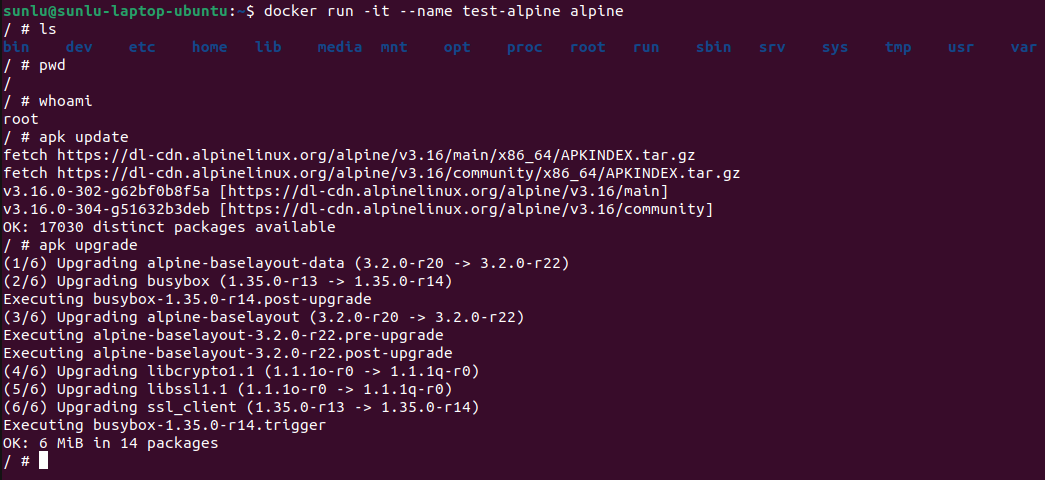
\includegraphics[width=350pt]{chapters/ch-virtualization-and-containerization/figures/dockerrunexp.png}
	\caption{An example of running \textit{apline} container, with interactive TTY and name \textit{test-apline}.} \label{ch:vac:fig:dockerrunexp}
\end{figure}

It can be seen from Fig. \ref{ch:vac:fig:dockerrunexp} that once the container is started, the user can interact with the container via shell, and perform actions such as listing items in the current directory in the container. While keeping the container running, open another terminal and use \verb|docker container ls|. The container \verb|test-alpine| shall appear in the list, as shown in Fig. \ref{ch:vac:fig:dockerrunexppart2}.
\begin{figure}
	\centering
	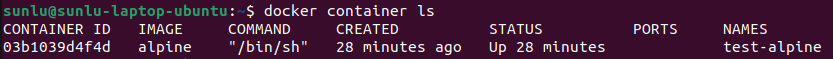
\includegraphics[width=250pt]{chapters/ch-virtualization-and-containerization/figures/dockerrunexppart2.png}
	\caption{List the running container \textit{test-apline}.} \label{ch:vac:fig:dockerrunexppart2}
\end{figure}

After exiting from Fig. \ref{ch:vac:fig:dockerrunexp} (by using \verb|exit| in \textit{alpine}), the container will transfer its status from ``running'' to ``exited'', as shown in Fig. \ref{ch:vac:fig:dockerrunexppart3}.
\begin{figure}
	\centering
	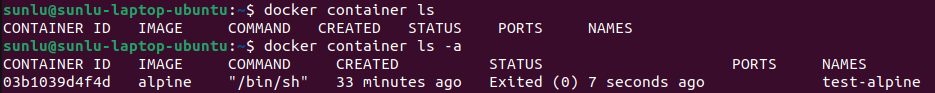
\includegraphics[width=250pt]{chapters/ch-virtualization-and-containerization/figures/dockerrunexppart3.png}
	\caption{List the exited container \textit{test-apline}.} \label{ch:vac:fig:dockerrunexppart3}
\end{figure}

It is also possible to launch a container and let it run in the backend using \verb|-d| flag. An example is given below.
\begin{lstlisting}
$ docker run -dt --name test-background-alpine alpine
\end{lstlisting}
By changing \verb|-i| to \verb|-d|, the container runs in the backend silently. The status of the container, after executing the above command, will stay running and can be displayed by \verb|docker container ls|.

Commonly used commands regarding launching a container are given in Tables \ref{ch:vac:tab:launchcontainer}, and \ref{ch:vac:tab:listcontainer}.

\begin{table}
	\centering \caption{Commonly used docker commands to launch a container.}\label{ch:vac:tab:launchcontainer}
	\begin{tabularx}{\textwidth}{llX}
		\hline
		Command & Flag & Description \\ \hline
		\verb|docker run| & --- & Launch a container of the image followed by the command. If the image cannot be found locally, it downloads the image from the remote repository automatically. Assign a random name to the container. Exit the container after execution. \\ \hdashline
        \verb|docker run| & \verb|-i| & Keep the standard input of the container open when launching the container. \\ \hdashline
        \verb|docker run| & \verb|-d| & Launch the container in the backend and keep it running. \\ \hdashline
        \verb|docker run| & \verb|-rm| & Automatically remove the container when exiting. The removed container will not be listed in \verb|docker container ls -a|. This is usually used for testing and debugging. \\ \hdashline
        \verb|docker run| & \verb|-t| & Allocate a pseudo-TTY. The flag usually comes with the flags \verb|-i| or \verb|-d|, to form \verb|-it| or \verb|-dt|. \\ \hdashline
        \verb|docker run| & \verb|--restart| & Enforce restart of the container upon exiting. This is usually used on containers running in the backend. Commonly used restart configurations include \verb|--restart no| (do not restart), \verb|--restart on-failure[:<max retries>]| (restart if exits with an error flag), \verb|--restart always| (always restart when exists). \\ \hdashline
        \verb|docker run| & \verb|--name| & Assign a name to the container. \\
		\hline
	\end{tabularx}
\end{table}

\begin{table}
	\centering \caption{Commonly used docker commands to display local images and containers.}\label{ch:vac:tab:listcontainer}
	\begin{tabularx}{\textwidth}{llX}
		\hline
		Command & Flag & Description \\ \hline
        \verb|docker image ls| & --- & List local images. \\ \hdashline
        \verb|docker container ls| & --- & List running containers. \\ \hdashline
        \verb|docker container ls| & \verb|-a| & List all containers. \\
		\hline
	\end{tabularx}
\end{table}

\subsection{Basic Container Management}

To start an exited container, use
\begin{lstlisting}
$ docker start <container>
\end{lstlisting}
This command starts the exited container, and keep it running in the backend.

For a container running in the backend, use \verb|docker exec| to execute a shell command in that container as follows.
\begin{lstlisting}
$ docker exec <container> <command>
\end{lstlisting}

To enable the TTY shell of a container running in the backend, use
\begin{lstlisting}
$ docker exec -it <container> <shell name>
\end{lstlisting}
Notice that the shell used by the application running inside the container may differ from the one used in the host machine. In the case of an \textit{alpine} image based container, \verb|ash| is the default shell. For a \textit{ubuntu} image based container, \verb|bash| is often used. To exit from the TTY shell while keep the container running in the backend, use shortcut key \verb|Ctrl+p+q|.

An alternative way to interact with containers running in the backend is to use
\begin{lstlisting}
$ docker attach <container>
\end{lstlisting}
to attach local standard input, output, and error streams to a running container. Similar with the previously introduced \texttt{docker exec -it} command, \texttt{docker attach} also starts the shell of the application running in the container. Use \verb|Ctrl-C| to quite the shell.

To check the processes that is running in the container, use
\begin{lstlisting}
$ docker top <container>
\end{lstlisting}

There are multiple ways and protocols to access with the files in a container, depending the I/O setup of the container. For a container running locally, \verb|docker cp| can be used for file transfer between the container and the host machine as follows. From container to host machine:
\begin{lstlisting}
$ docker cp <container>:<source> <destination>
\end{lstlisting}
and from host machine to container:
\begin{lstlisting}
$ docker cp <source> <container>:<destination>
\end{lstlisting}
where \verb|<source>| and \verb|<destination>| refer to the path to the source and destination, respectively, located in the host machine or the container.

To stop, kill (force stop) or restart a container running in the backend, use
\begin{lstlisting}
$ docker stop <container>
$ docker kill <container>
$ docker restart <container>
\end{lstlisting}
respectively. When a container is stopped, it enters exited status. To remove an exited container or all exited containers, use
\begin{lstlisting}
$ docker container rm <container>
\end{lstlisting}
or
\begin{lstlisting}
$ docker container prune
\end{lstlisting}
respectively. To rename a container (without changing its container ID or anything else), use
\begin{lstlisting}
$ docker rename <container-old-name> <container-new-name>
\end{lstlisting}

To quickly check container status (CPU, memory usage, etc.) of a running container or all running containers, use
\begin{lstlisting}
$ docker stats <container>
\end{lstlisting}
where the container name can be specified as an option. To list down more detailed information of a container, including its status, gateway, IP address, etc., use
\begin{lstlisting}
$ docker inspect <container>
\end{lstlisting}
Finally, to check the logs of a container (e.g., its standard output to the console), use
\begin{lstlisting}
$ docker logs <container>
\end{lstlisting}

A container is usually generated from its image. It is also possible to package a container into an image. To create an image from a container, use
\begin{lstlisting}
$ docker commit <container> <image>
\end{lstlisting}
where \verb|docker commit| command saves the container's file changes or settings into a new image, which allows easier populating containers or debugging in a later stage. Notice that \verb|docker commit| does not save everything of the container into the image, and it is not the only way an image is created.

\subsection{Example: A Web Server}

A container can be configured accessible from not only the host machine but also other computers in LAN or the Internet. In a typical web service application, the host machine and the containers are often designed following the architecture similar with Fig. \ref{ch:vac:fig:containerwebserverarchitecture}. Notice that in practice, the load balancer and the containers may or may not run on the same physical machine.

The load balancer is a container orchestration that monitors the status of the containers, manages the data flow, and scales up and down the number of containers depending on the total load. In case where there are multiple physical servers, the load balancer is run on a ``master'' server, and the containers are distributed on multiple ``slave'' servers, each of which is called a ``worker node'', or ``node'' for simplicity. Container engines are installed on each and every node. The load balancer talks with the container engines on each node to deploy containers. The APP, in this case a web servers such as \textit{apache} or \textit{nginx}, shall run in the containers.
\begin{figure}
	\centering
	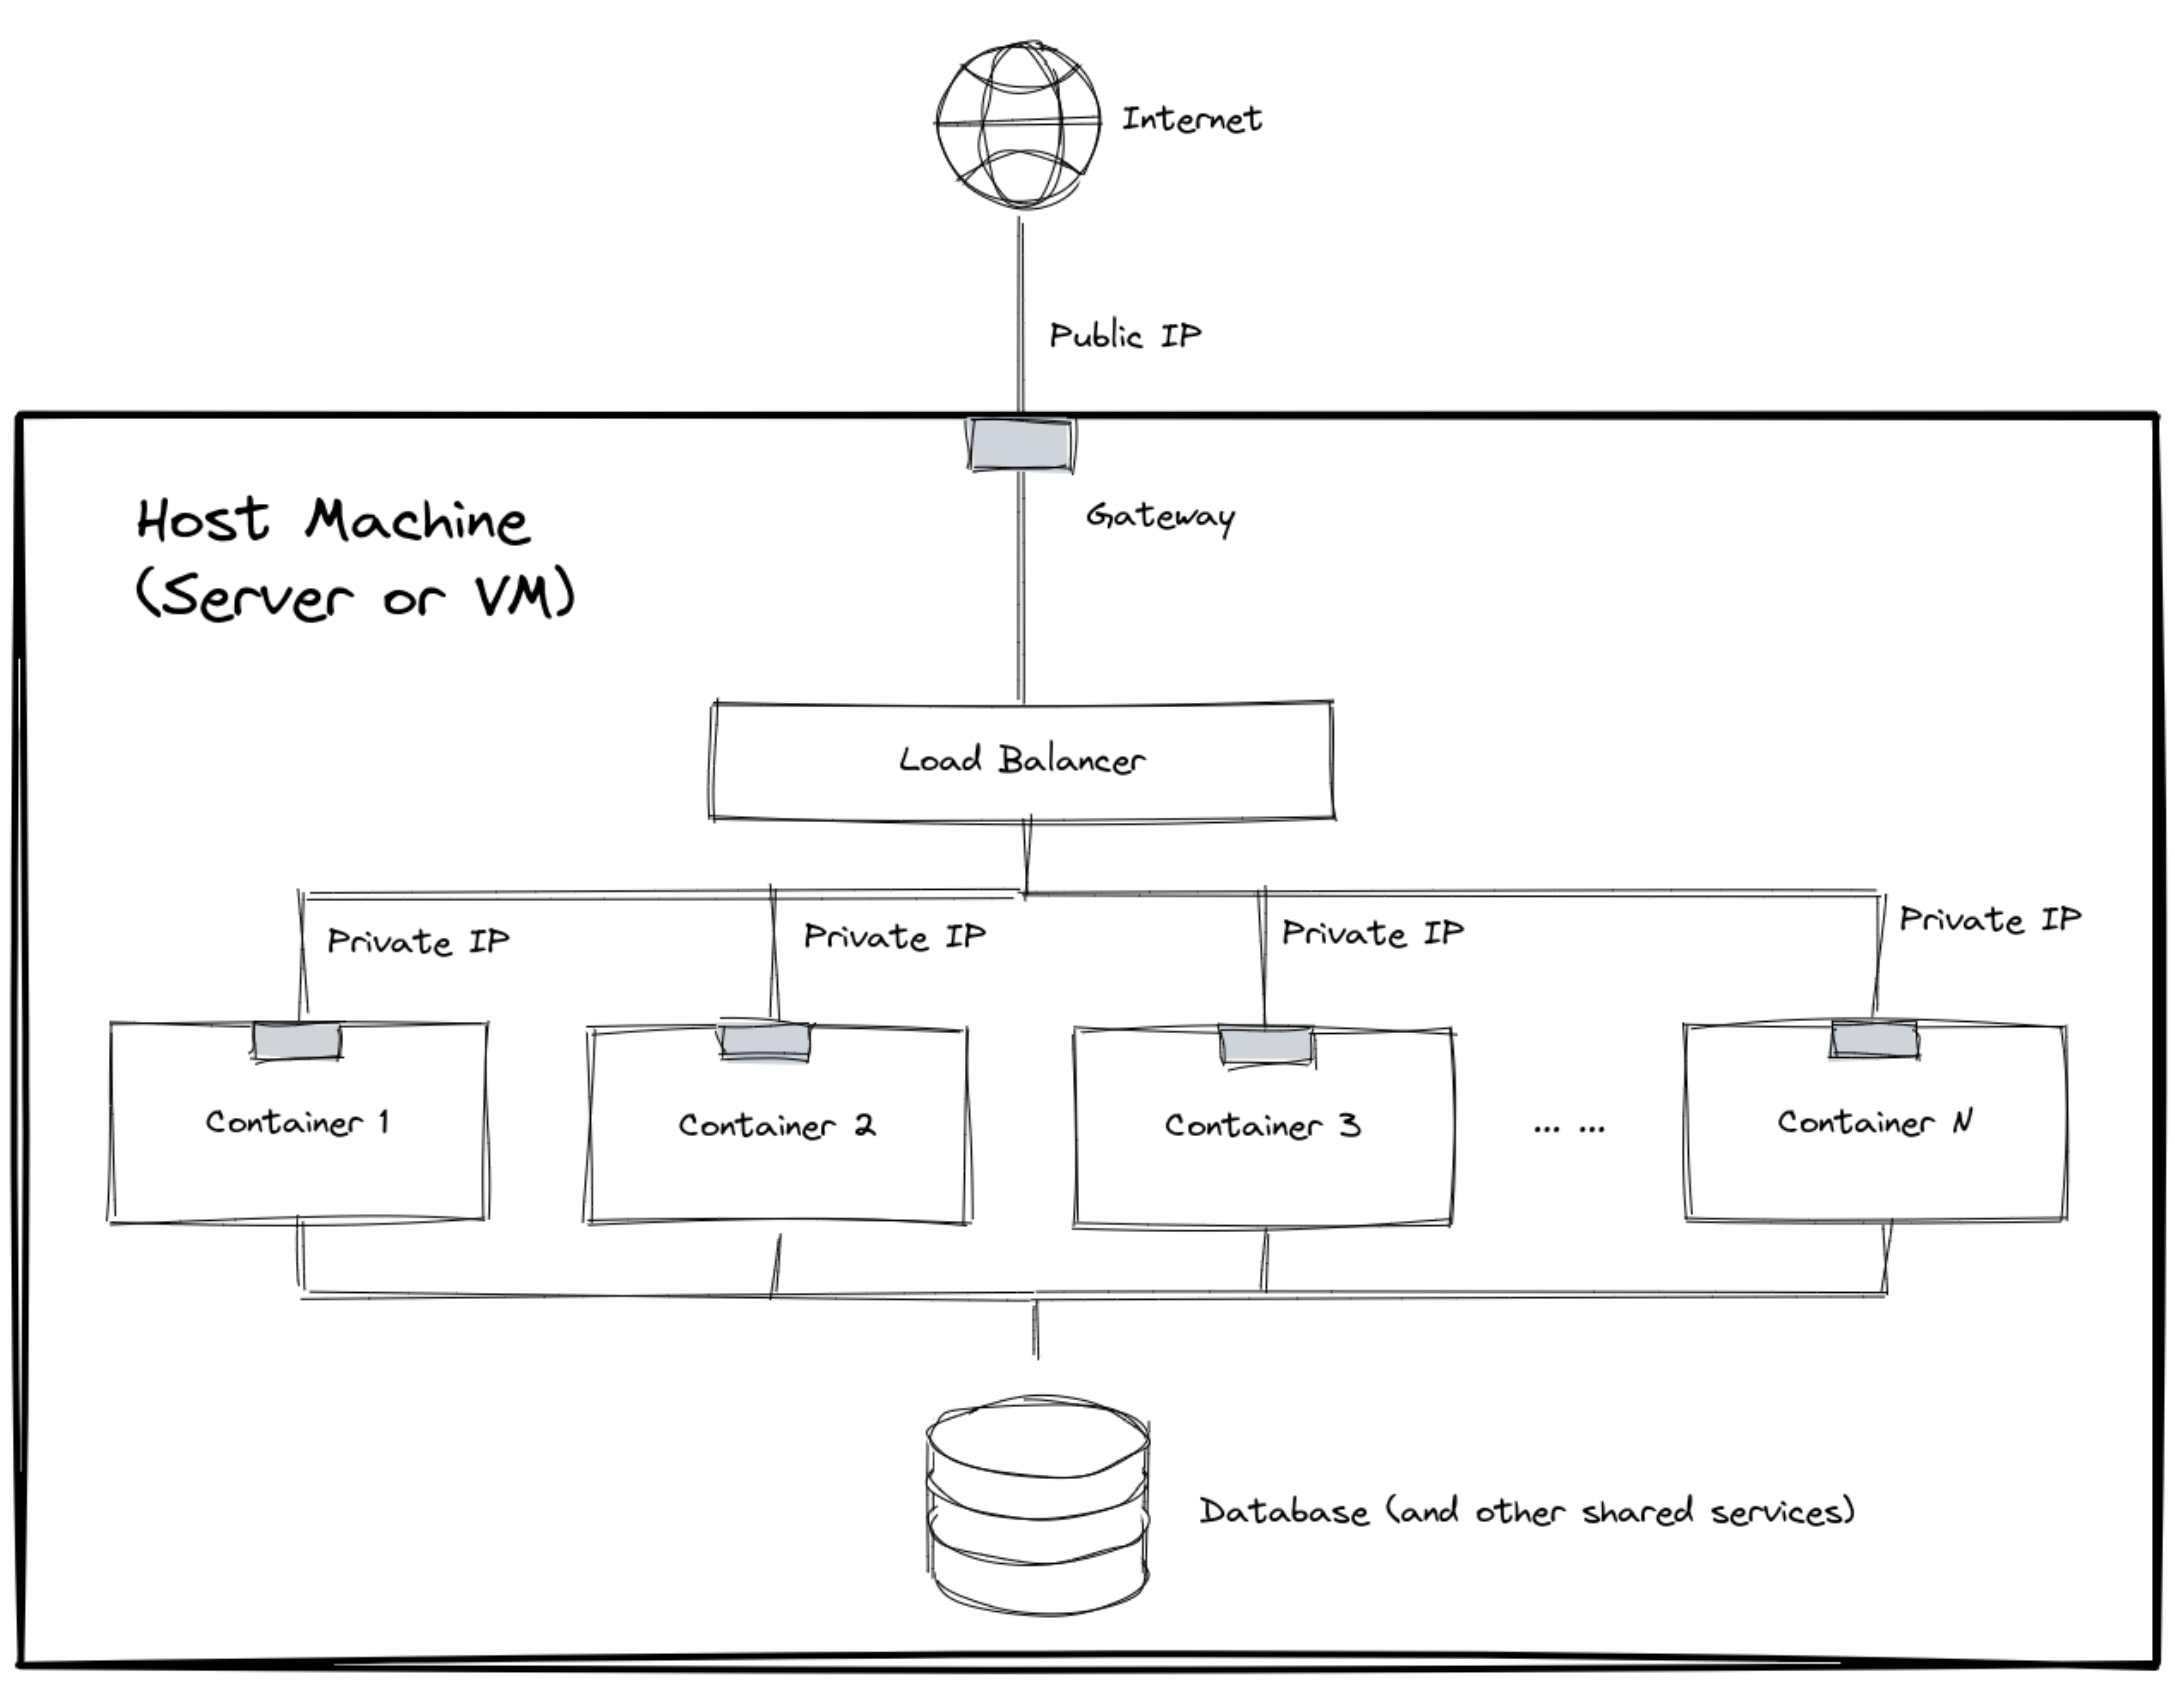
\includegraphics[width=350pt]{chapters/ch-virtualization-and-containerization/figures/containerwebserverarchitecture.png}
	\caption{A simplified architecture where containers are used to host the web service.} \label{ch:vac:fig:containerwebserverarchitecture}
\end{figure}

An example of setting up a web server in containers from scratch is given in this section. For simplicity, everything is on a single physical server. Only one container is used and the load balancer and the shared services are not included in the example. As a first step, create a container from the official \textit{nginx} image as follows. Notice that it is also possible to create a container from \textit{apline}, and install \textit{nginx} on \textit{apline}.
\begin{lstlisting}
$ docker run -dt --name simple-web nginx
\end{lstlisting}

Next, create the configuration file for \textit{nginx}, and also the \textit{html} files to be used as the static web page. For convenience, the files are created and edited in the host machine, then copied to the container. The following \textit{default.conf} and \textit{index.html} have been created, respectively. The configuration file \textit{default.conf}:
\begin{lstlisting}
server {
	listen 80 default_server;
	listen [::]:80 default_server;
	root /var/www/html/;
}
\end{lstlisting}
The \textit{html} file \textit{index.html}:
\begin{lstlisting}
<html>
	<body>
		<h1>Hello World!</h1>
	</body>
</html>
\end{lstlisting}
Use \verb|docker copy| to copy the two files to the designed locations in the container as follows.
\begin{lstlisting}
$ docker exec simple-web mkdir /var/www
$ docker exec simple-web mkdir /var/www/html
$ docker cp default.conf simple-web:/etc/nginx/conf.d/default.conf
$ docker cp index.html simple-web:/var/www/html/index.html
\end{lstlisting}
Change the ownership of the \textit{html} file as follows, so that the current user \textit{nginx} is able to access that file.
\begin{lstlisting}
$ docker exec simple-web chown -R nginx:nginx /var/www/html
\end{lstlisting}

Finally, reload and configuration file and restart the web server as follows.
\begin{lstlisting}
$ docker exec simple-web nginx -s reload
\end{lstlisting}

To test the web server running inside the container, obtain the IP address of the container using
\begin{lstlisting}
$ docker inspect simple-web | grep IPAddress
\end{lstlisting}
and open a browser with the obtained IP address keyed in. If everything is done correctly, the browser should try to access port 80 of the container, and the ``Hello World!'' web page shall show up.

For easy sharing and populating of the container, commit the container into a new image using \verb|docker commit| as follows. The new image can be used to populate the web server, just like ``web01'' container given below.
\begin{lstlisting}
$ docker commit simple-web simple-web-image
$ docker run -dt --name web01 -p 80:80 simple-web-image
\end{lstlisting}
where \verb|-p <host machine port>:<container port>| is used to map ports. Notice that different from the previous container ``\textit{simple-web}'', the new container ``\textit{web01}'' IP address port 80 is mapped with the port 80 of the host machine. Therefore, the web page hosted in ``\textit{web01}'' can be accessed not only by the container's IP address, but also by the host machine IP address. Key in \verb|localhost| in the browser on the host machine and the ``Hello World!'' web page shall show up.

\subsection{Docker Volume}

As introduced earlier, \verb|docker cp| can be used to transfer data into and out of a container. Alternatively, Docker volumes can be used, which is more convenient when there are massive data to be transferred frequently. 

Docker volumes are the mapping of disk storage from outside the container to inside. With Docker volume, the data inside the container can be backed up, migrated, or shared among containers easily. Docker volume is critical for some applications, such as a database. To create a volume, use
\begin{lstlisting}
$ docker volume create <volume>
\end{lstlisting}
To list down volumes and to inspect a volume, use
\begin{lstlisting}
$ docker volume ls
$ docker volume inspect <volume>
\end{lstlisting}
respectively. Finally to remove a volume or all volumes, use
\begin{lstlisting}
$ docker volume rm <volume>
$ docker volume prune
\end{lstlisting}
respectively.

When starting a container from an image, volumes can be mapped with the internal storage inside the container by using
\begin{lstlisting}
$ docker run -v <volume>:<container-internal-path>[:ro] <image>
\end{lstlisting}
which should synchronize \verb|<volumn name>| with \verb|<container internal path>|. The optional \verb|:ro| can be specified if it is a read-only volume. Instead of using a volume name, the path to a directory in the host machine can also be used, in which case the specified directories in the host machine and in the container should be synchronized.

Notice that the data persists in the host machine, and in the container it is taken as a mounted volume. Therefore, synchronized files does not duplicate physically, and the data persists and remains accessible after removing the container.

\section{Docker Image} \label{ch:vac:sec:di}

In earlier Section \ref{ch:vac:sec:dc}, images have been used to create containers. An image performs like a template or source of a container. It contains information regarding the basic settings, initial configurations, required libraries, and other metadata of the container. Images can be shared across different machines and platforms. More details about the formulation and function of a docker image are introduced in the rest of this section.

\subsection{Image Architecture}

An image shall contain everything needed to create and initialize a container. This include but not limited to:
\begin{itemize}
  \item Necessary steps (also known as ``layers'') to create a container.
  \item Application code that is to run in the containers
  \item Files to support the application
  \item Libraries, tools and dependencies
\end{itemize}
In addition, an image shall be designed and organized in such a way that it is migratable, reusable and light, and can be used to easily populate large number of containers. For better inheritability, an image might be based on another existing image, which is called its parent image. An image with no parent, such as the official \textit{hello-world} image from Docker Hub, is called a base image.

\subsection{Dockerfile}

Dockerfile is a human-readable text document that serves as an instruction for building a Docker image, as shown in Fig. \ref{ch:vac:fig:dockerfiletoimage}. Notice that the Dockerfile itself is not included in the image it built.

\begin{figure}
	\centering
	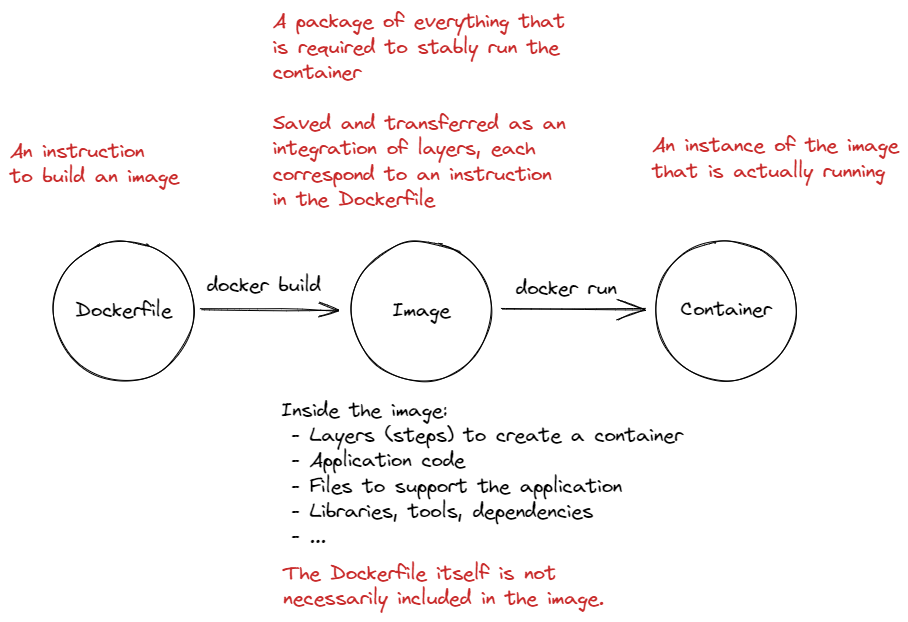
\includegraphics[width=350pt]{chapters/ch-virtualization-and-containerization/figures/dockerfiletoimage.png}
	\caption{A demonstration of how Dockerfile, image and container link to each other.} \label{ch:vac:fig:dockerfiletoimage}
\end{figure}

Since a Docker image is mainly used as a container template, many commands in a Dockerfile reads like a ``step-by-step'' instructions of creating a container, with each instruction correspond to a ``layer'' in the image. An image can be regarded as an integration of multiple layers, and it is indeed stored and shared in that way. For images that share layers (for example, two images of different versions of the same APP), the shared layers will not be saved or transferred in a duplicated manner. This largely reduces the weight of an image. More details are given on \textit{https://docs.docker.com/storage/storagedriver/}.

Docker containers use a special filesystem called Union File System (UFS), which aligns well with the ``layer'' concept. The UFS provides useful features such as enabling file sharing between the container and the host machine, and integrating read-only upper layers and writable lower layers, etc.

A demonstration to illustrate this concept is given later in Fig. \ref{ch:vac:fig:dockerlayerdemo}.


Just as a quick example, the Dockerfile to build the official \textit{hello-world} image from Docker Hub looks like the following.
\begin{lstlisting}
FROM scratch
COPY hello /
CMD ["/hello"]
\end{lstlisting}
Similar with other computer languages, Dockerfile has reserved keywords, environmental variables, syntax and grammar rules. Only the basics of forming a Dockerfile is introduced in this section. More details can be found in the docker reference from the official website. In the example above, \verb|FROM scratch| indicates that this image is a base image without a parent. The following \verb|COPY hello /| suggests to copy the \textit{hello} binary script from the image to the root directory. Finally, \verb|CMD ["/hello"]| executes \textit{hello} binary script.

Generally speaking, a typical Dockerfile shall consist of the following instructions in order to build an image. With these instructions, the image would know how to create a container and automatically build filesystem directory structure, install necessary packages, and run the APP.
\begin{enumerate}[(1)]
  \item Define parent image.
  \item Create filesystem directory.
  \item Set working directory.
  \item Copy files.
  \item Configure registry.
  \item Install packages.
  \item Copy more files after the packages installation.
  \item Switch to the correct user.
  \item Expose port.
  \item Run the APP.
\end{enumerate}

The keywords to be used in a Dockerfile to realize the above instructions, such as \verb|FROM|, \verb|RUN|, and many more, are explained in Table \ref{ch:vac:tab:keywordsdockerfile}.

\begin{table}
	\centering \caption{Critical keywords used in a Dockerfile.}\label{ch:vac:tab:keywordsdockerfile}
	\begin{tabularx}{\textwidth}{lX}
		\hline
		Syntax & Description \\ \hline
		\verb|FROM <image>| & Define the parent image. A Dockerfile must start with a \verb|FROM| instruction. A Dockerfile can contain multiple \verb|FROM| instruction, in which case the last \verb|FROM| statement is the final base image and the earlier \verb|FROM| instructions creates intermediate images that can be used in the final image. An optional \verb|:<tag>| following \verb|<image>| can be used to specify the version of the image to use as the base. By default, the latest version of the image will be used. \\ \hdashline
		\verb|RUN <command>| & Execute a shell command using \verb|/bin/sh -c|. \\ \hdashline
		\verb|WORKDIR <path>| & Set the working directory from the point onwards. This is often a preparation for the upcoming \verb|RUN|, \verb|COPY|, etc., commands. \\ \hdashline
		\verb|ADD <src> <dest>| & Add \verb|<src>|, either a directory/file or URL, to \verb|<dest>|. An optional \verb|[--chown=<user>:<group>]| can be used to specify the owner and group of the added files. \\ \hdashline
		\verb|COPY <src> <dest>| & Copy \verb|<src>|, a directory/file, to \verb|<dest>|. An optional \verb|[--chown=<user>:<group>]| can be used to specify the owner and group of the added files. Notice that \verb|COPY| is similar with \verb|ADD|, just easier to use but in return less powerful. \\ \hdashline
		\verb|USER <user>| & Switch user for the instructions beyond this point. \\ \hdashline
		\verb|EXPOSE <port>| & Specifies the ports that the container shall listen to. An optional \verb|/<protocol>| following \verb|<port>| can be used to specify the protocol for communication. \\ \hdashline
		\verb|CMD ["<exe>", "p1", ...]| & As the last instruction of a Dockerfile, run the APP. Notice that a Dockerfile can only contain one \verb|CMD| instruction. The executable command name and the parameters are put into a list. \\
		\hline
	\end{tabularx}
\end{table}

Besides Table \ref{ch:vac:tab:keywordsdockerfile}, there are other Dockerfile keywords that can significantly convenient the design and maintenance of the image. For example, \verb|ENV <key>=<value>| assign a value to an environmental variable; \verb|LABEL <key>="<value>"| assigns a tag to the image, which can be displayed when \verb|docker inspect <container>| is used.

Examples of Dockerfiles are given below, one from \textit{docs.docker.com} and the other from Linux Academy.

The docker image layer structure of the second example is given in Fig. \ref{ch:vac:fig:dockerlayerdemo} as a demonstration. Notice that in Fig. \ref{ch:vac:fig:dockerlayerdemo}, \verb|bootfs| refers to the ``boot file system'', including the bootloader and the Linux kernel. Upon run, a container layer will be added to the image, as shown by the blue dashed box in Fig. \ref{ch:vac:fig:dockerlayerdemo}. In the container, all the changes made is saved into the container layer.

To generate a new image to include the changes made in the container, use \verb|docker commit|, which essentially commits the container layer as the latest image layer in the new image, as shown by the green dashed box in Fig. \ref{ch:vac:fig:dockerlayerdemo}.

\begin{lstlisting}
# First Example
FROM golang:1.16
WORKDIR /go/src/github.com/alexellis/href-counter/
RUN go get -d -v golang.org/x/net/html
COPY app.go ./
RUN CGO_ENABLED=0 GOOS=linux go build -a -installsuffix cgo -o app .

FROM alpine:latest
RUN apk --no-cache add ca-certificates
WORKDIR /root/
COPY --from=0 /go/src/github.com/alexellis/href-counter/app ./
CMD ["./app"]
\end{lstlisting}

\begin{lstlisting}
# Second Example
FROM node:10-alpine
RUN mkdir -p /home/node/app/node_modules && chown -R node:node /home/node/app
WORKDIR /home/node/app
COPY package*.json ./
RUN npm config set registry http://registry.npmjs.org/
RUN npm install
COPY --chown=node:node . .
USER node
EXPOSE 8080
CMD ["node", "index.js"]
\end{lstlisting}

\begin{figure}
	\centering
	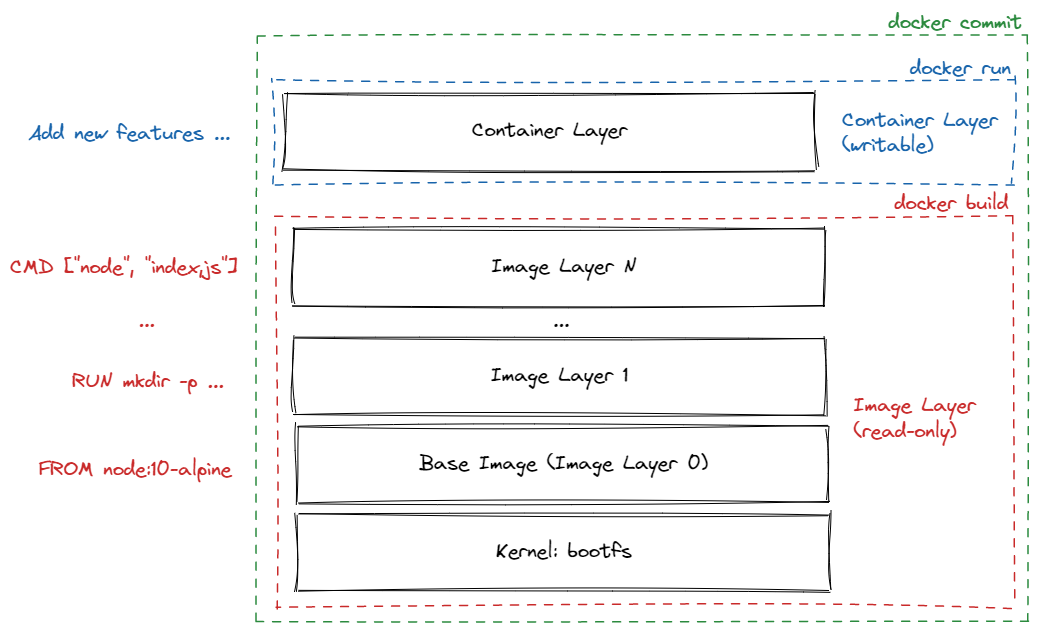
\includegraphics[width=350pt]{chapters/ch-virtualization-and-containerization/figures/dockerlayerdemo.png}
	\caption{A demonstration of docker image layer structure using the aforementioned example.} \label{ch:vac:fig:dockerlayerdemo}
\end{figure}

With the Dockerfile ready, use \verb|docker build| to build an image. An example is given as follows.
\begin{lstlisting}
$ docker build <path/url> -t <image name>
\end{lstlisting}
where \verb|<path/url>| is the path or URL to the directory where the Dockerfile locates (does not need to contain ``\verb|/Dockerfile|'' in its end), and \verb|-t| gives a tag, in this case an image name, to the image to build.

\subsection{Docker Image Operations}

The most commonly used image operations can be categorized as follows.
\begin{itemize}
  \item Create an image.
  \item Create a container from an image.
  \item Upload and download an image from a remote server.
  \item Manage local images, such as listing down all images, deleting an image, etc.
\end{itemize}

The first two categories have been introduced in earlier sections. The third and last categories are introduced as follows.

Use the following command to search for an image on the default remote repository server (Docker Hub).
\begin{lstlisting}
$ docker search <image name>
\end{lstlisting}

Use the following command to download or update an image from the default remote repository server as follows. Notice that different from \verb|docker run|, this command will not start a container from the image.
\begin{lstlisting}
$ docker pull <image name>
\end{lstlisting}
There is one thing to highlight about \verb|docker pull|. Notice that since an image is stored by layers, if another image that shares some layers with the image to be downloaded already exists, the shared layers will not be downloaded again to avoid duplication.

Use the following commands to list down or remove images as follows.
\begin{lstlisting}
$ docker image ls
$ docker image rm <image name>
$ docker image prune # remove all problematic images
$ docker image prune -a # remove all unused images
\end{lstlisting}
where \verb|prune| removes all problematic images, and \verb|prune -a| removes all unused images from local.

Use the following command to inspect an image, and list down its metadata details.
\begin{lstlisting}
$ docker image inspect <image name>
\end{lstlisting}

\section{Advanced Container Management Using Portainer}

Docker is a great tool to build and share images, and to create containers from images. It is introduced from earlier sections that Docker can also monitor and manage the running containers in a simple manner, for example checking the status of the containers using \verb|docker container ls|, and stopping a container using \verb|docker stop <container name>|.

However, the container management functions built-in with Docker may not be powerful and flexible enough in some occasions. Thus, more advanced container management tools have emerged, some of which integrated with useful features such as auto-scaling the number of the running containers. These container management tools are often used collaboratively with Docker: Docker builds images and creates containers, while the container management tools manage the running of the containers. As one of the many container management tools, \textit{Portainer} is introduced in this section.

Portainer is an open-source container management tool, and it is free-of-charge for personal usage. It has a web-based UI and puts everything into a dashboard. Notice that Protainer itself also runs in a container, hence can be managed just like any other container.

Before starting a Portainer container, it is a good practice to first create a Docker volume for Portainer to store the database. Use the following command to create such Docker volume.
\begin{lstlisting}
$ docker volume create portainer_data
\end{lstlisting}
Then run a Protainer container using
\begin{lstlisting}
$ docker run -d -p 8000:8000 -p 9000:9000 -p 9443:9443 --name portainer --restart=always -v /var/run/docker.sock:/var/run/docker.sock -v portainer_data:/data portainer/portainer-ce
\end{lstlisting}
where ports 8000, 9000 and 9443 are used for development environments of web server software, management server service, and SSL, respectively. It is often possible to ignore \verb|-p 9000:9000| unless for legacy reasons.  The \verb|docker.sock| is the socket that enables the docker server-side daemon to communicate with its command-line interface. The image name for Portainer community edition (distinguished form the business edition) is \verb|portainer/portainer-ce|.

Use \verb|https://localhost:9443| to login to the container. The following page in Fig. \ref{ch:vac:fig:portainerlogin} should pop up in the first-time login, requiring to add an admin user.
\begin{figure}
	\centering
	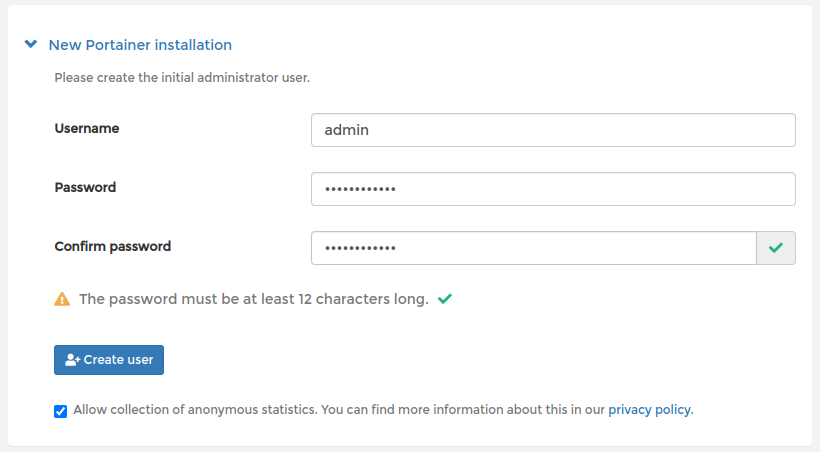
\includegraphics[width=350pt]{chapters/ch-virtualization-and-containerization/figures/portainerlogin.png}
	\caption{Portainer login page to create admin user.} \label{ch:vac:fig:portainerlogin}
\end{figure}

After creating the admin user and logging in, the status of images, containers and many more can be monitored via the dashboard, as shown in Figs. \ref{ch:vac:fig:portainerdashboard1}, \ref{ch:vac:fig:portainerdashboard2} and \ref{ch:vac:fig:portainerdashboard3}. Notice that in Fig. \ref{ch:vac:fig:portainerdashboard3}, using the ``quick action'' buttons, the user can check the specifics of the container and interact with its console, just like using \verb|docker container inspect| and \verb|docker exec|
\begin{figure}
	\centering
	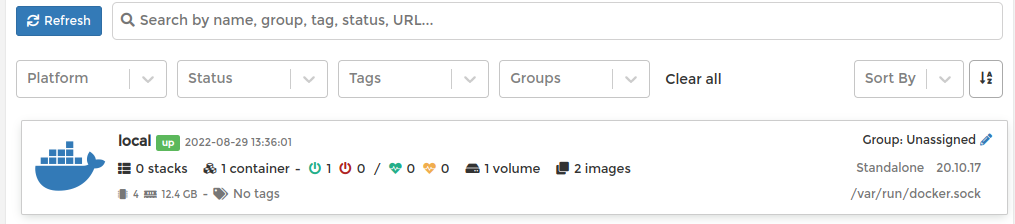
\includegraphics[width=350pt]{chapters/ch-virtualization-and-containerization/figures/portainerdashboard1.png}
	\caption{Portainer dashboard overview of docker servers.} \label{ch:vac:fig:portainerdashboard1}
\end{figure}

\begin{figure}
	\centering
	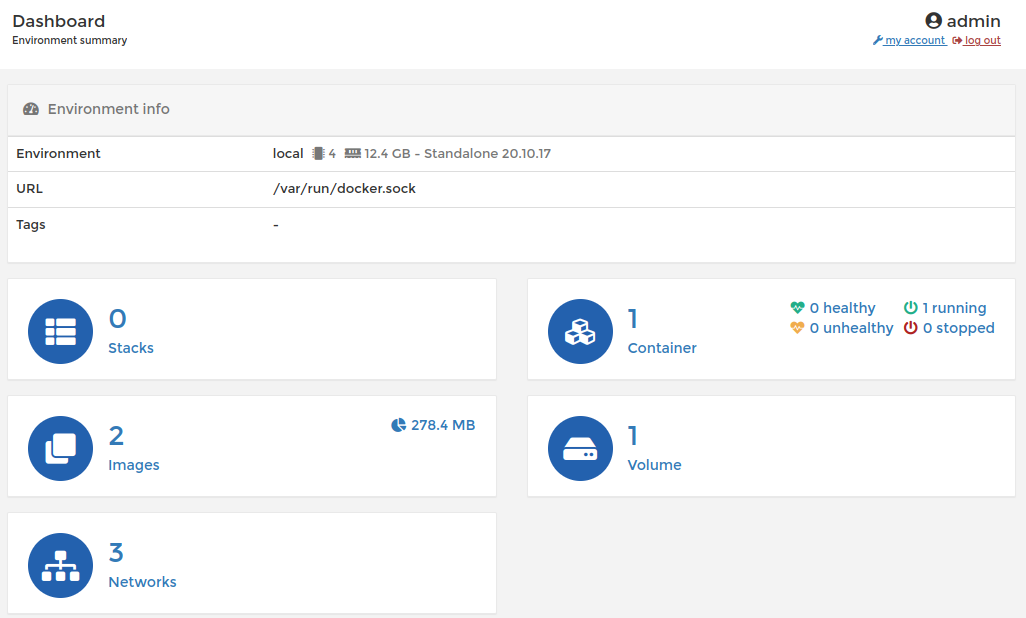
\includegraphics[width=350pt]{chapters/ch-virtualization-and-containerization/figures/portainerdashboard2.png}
	\caption{Portainer dashboard overview in a docker server.} \label{ch:vac:fig:portainerdashboard2}
\end{figure}

\begin{figure}
	\centering
	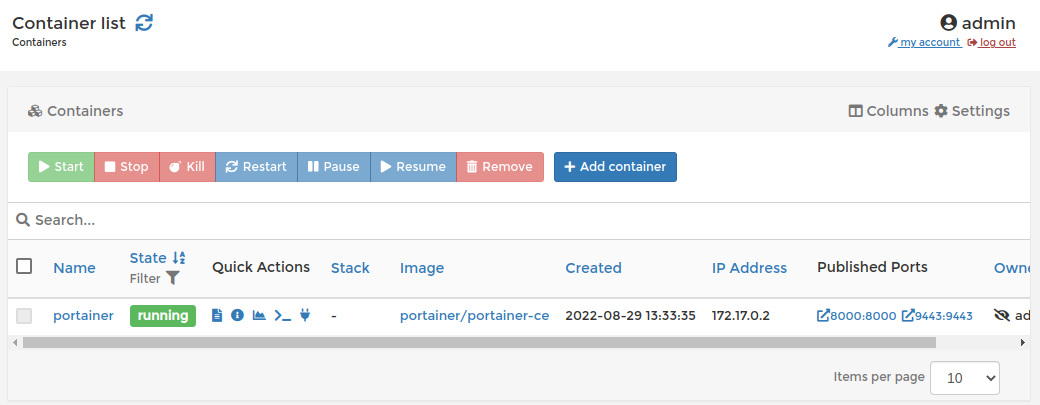
\includegraphics[width=350pt]{chapters/ch-virtualization-and-containerization/figures/portainerdashboard3.png}
	\caption{Portainer dashboard list down of all running containers.} \label{ch:vac:fig:portainerdashboard3}
\end{figure}

In summary, Portainer provides an easy-to-use container management tool with clean graphical interface that a user can quickly get used to without a steep learning curve.

\section{Advanced Container Management Using Kubernetes}

\textit{Kubernetes}, also known as \textit{k8s}, is an open-source container orchestration system originally developed by Google for automating deployment, scaling and management of containerized applications, guaranteeing their high availability and resilience. By default, Kubernetes command line tool, \textit{kubectl}, is used to interact with Kubernetes and manage the containers. Kubernetes is more powerful than Portainer, but at the same time more complicated and difficult to use.

Figure \ref{ch:vac:fig:kubernetescluster} demonstrates a Kubernetes cluster and how its key components are managed inside the cluster.
\begin{figure}
	\centering
	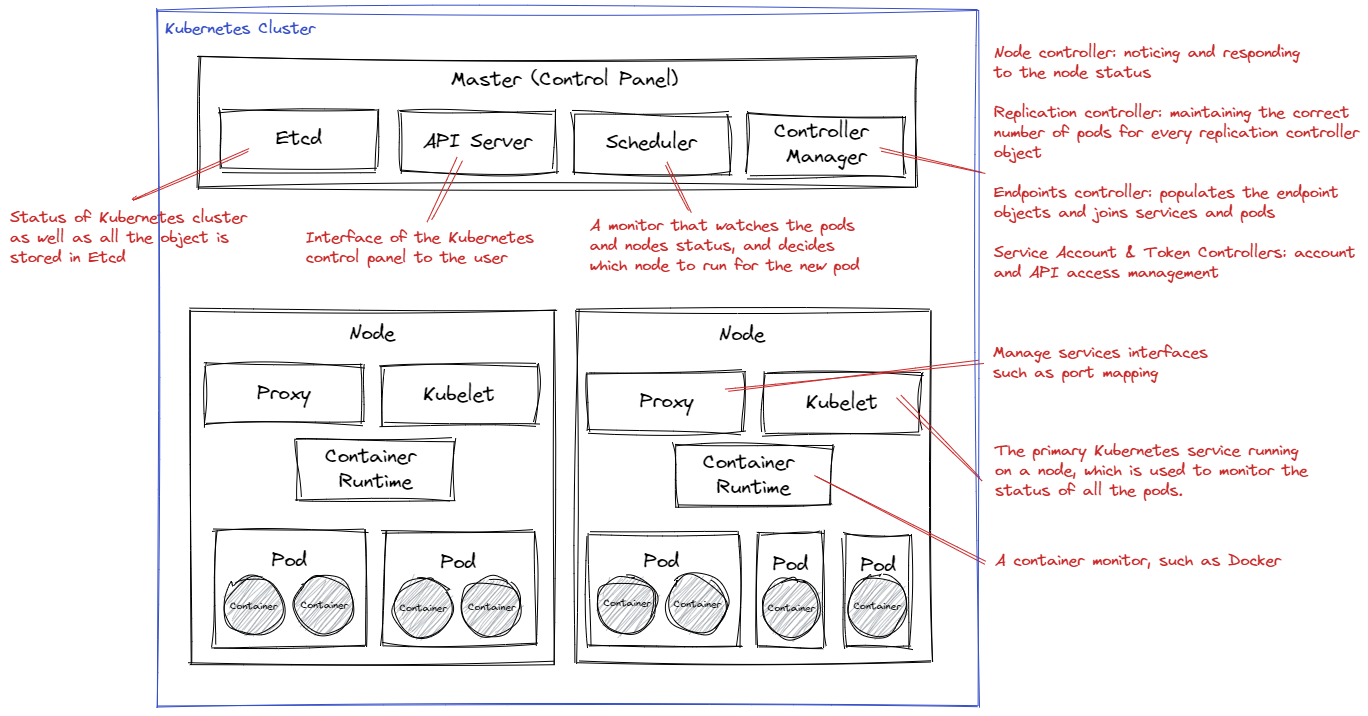
\includegraphics[width=350pt]{chapters/ch-virtualization-and-containerization/figures/kubernetescluster.png}
	\caption{Kubernetes cluster and its key components.} \label{ch:vac:fig:kubernetescluster}
\end{figure}

As shown in Fig. \ref{ch:vac:fig:kubernetescluster}, Kubernetes manages containers in a centralized ``master-worker (node)'' mode, where the master also plays as the control panel, API gateway (with static IP address) and load balancer to interact with a user. 

In practice, the master and nodes can run on multiple servers or VMs. Kubernetes packages need to be installed on all these servers or VMs for the system to work properly. Kubernetes provides variety of tools to distribute the loads to different servers or VMs, or to add redundancy to the system for high availability. 

\subsection{Kubernetes Installation}

The installation guidance of kubernetes can be found at \textit{https://kubernetes.io/docs/setup/}. Key steps are summarized as follows.

\subsection{Kubernetes Practice}


In a production environment, a kubernetes cluster may look like the following.

\subsection{Kubernetes with Rancher}

\textit{Rancher}, just like Portainer, is an open-source container management tool that has a web-based UI and is relatively easy to use. Rancher can be used stand-alone just like Portainer. What makes Rancher special is that it can help to deploy and manage Kubernetes, which essentially adds an additional UI layer to Kubernetes and makes its use easier. Therefore, by using Rancher together with Kubernetes as a whole, we can have a powerful yet user-friendly container management approach.

\section{Docker Hub}

Docker Hub is a commonly used server for storing and sharing docker images. It is also the default remote repository server of Docker engine. However, do notice that Docker Hub is not the only remote docker image server. Some alternatives are Amazon Elastic Container Registry, Red hat Quay, Azure Container Registry, Google Container Registry, etc.

After registering an account on Docker Hub, use the following command to login to the docker hub from your local machine.
\begin{lstlisting}
$ docker login --username=<user name>
Passowrd:
\end{lstlisting}

Assume that there is an image in the local machine, and an empty repository on Docker Hub. In order to push the local image to the Docker Hub, the first step is to add the remote repository ad the ``\textit{RepoTags}'' in the local image as follows.
\begin{lstlisting}
$ docker tag <image name> <username>/<repository name>:<version>
\end{lstlisting}
where \verb|<version>| is a tag usually used to distinguish the different branches or versions of the images on Docker Hub. For the first image upload, it can simply be \verb|latest|.

Use the following command to push the image to Docker Hub.
\begin{lstlisting}
$ docker push <user name>/<repository name>
\end{lstlisting}




